% MAST30027 Modern Applied Statistics -- full mock exam (questions only)
\documentclass[11pt,a4paper]{article}
\usepackage[a4paper,portrait,top=2.4cm,bottom=2.2cm,left=2.2cm,right=2.2cm,headheight=14pt]{geometry}
\usepackage{fontspec}
\usepackage{amsmath,amssymb,mathtools}
\usepackage{fancyvrb}
\usepackage{fancyhdr}
\usepackage{enumitem}
\usepackage{graphicx}
\usepackage{needspace}
\usepackage{lastpage}
\usepackage{array,booktabs}
\setmonofont{lmmonolt10-regular.otf}[BoldFont=lmmonolt10-bold.otf,ItalicFont=lmmonolt10-oblique.otf]
\setlength{\parindent}{0pt}
\setlength{\parskip}{4pt}
\emergencystretch=3em
\clubpenalty=10000 \widowpenalty=10000
\pagestyle{fancy}
\fancyhf{}
\renewcommand{\headrulewidth}{0.4pt}
\fancyhead[L]{MAST30027 Modern Applied Statistics}
\fancyhead[R]{Semester 2, 2026}
\fancyfoot[C]{Page \thepage\ of \pageref{LastPage}}
\setlist[enumerate,1]{label=(\alph*),leftmargin=2em,itemsep=4pt,topsep=2pt}
\setlist[enumerate,2]{label=(\roman*),leftmargin=2em,itemsep=2pt,topsep=2pt}

\newcommand{\mk}[1]{\hfill\hspace*{\fill}\mbox{\,[#1~\ifnum#1=1 mark\else marks\fi]}}
\newcommand{\ans}[1]{\par\nopagebreak[4]\vspace{2pt}\noindent\fbox{\rule{0pt}{#1}\hspace{\dimexpr\linewidth-2\fboxsep-2\fboxrule\relax}}\par\vspace{4pt}}
\newcommand{\qhead}[2]{\Needspace{10\baselineskip}\vspace{10pt}{\large\bfseries Question #1 (#2 marks)}\par\vspace{2pt}}
\newcommand{\R}[1]{\VerbatimInput[fontsize=\footnotesize,frame=single,framesep=2mm,rulecolor=\color{black!50}]{final/r/out/#1}}
\usepackage{xcolor}
\renewcommand{\R}[1]{\VerbatimInput[fontsize=\scriptsize,frame=single,framesep=1.5mm,rulecolor=\color{black!50}]{r/out/#1}}
\DeclareMathOperator{\E}{\mathbb{E}}
\DeclareMathOperator{\Var}{Var}

\begin{document}
\thispagestyle{empty}
\begin{center}
\fbox{\parbox{0.95\linewidth}{\large Student ID: \hspace{6cm} Seat number: \rule[-2pt]{2.5cm}{0pt}\\[4pt]}}

\vspace{1.2cm}
{\Large\bfseries Semester 2 Exams, 2026}\\[6pt]
{\large School of Mathematics and Statistics}\\[1.2cm]
{\LARGE\bfseries MAST30027\_26\_SM2 -- Modern Applied Statistics}\\[1.0cm]
{\Large \textbf{MOCK PAPER}}\\[1.0cm]
{\large Reading time: 15 minutes\\[4pt] Writing time: 3 hours}
\end{center}
\vspace{1.0cm}

\textbf{Permitted materials}
\begin{itemize}[itemsep=1pt,topsep=2pt]
\item Pencils, pens, erasers, highlighters.
\item Calculator: Casio FX-82 (any suffix), non-programmable.
\item Student notes: 1 $\times$ double-sided A4 page of notes.
\end{itemize}

\textbf{Exam instructions}
\begin{itemize}[itemsep=1pt,topsep=2pt]
\item This paper contains \textbf{9 questions worth 78 marks}. Marks for each part are shown in square brackets.
\item During reading time you may not write, type, or select answers.
\item Show all working. Answers without supporting calculations or explanation may receive no marks.
\item Give numerical answers to \textbf{2 decimal places} unless the question says otherwise.
\item You will not be asked to write R code. R code and output are shown only so that you can read, interpret and compute from them. The output is real R output.
\item If you need more space, use the pages at the back of the paper and note this in the answer box.
\item The probability density and mass functions of the distributions on the next page are not repeated in the questions. Densities of other distributions (Binomial, Beta, etc.) are given only where a question needs them.
\end{itemize}

\vspace{0.6cm}
\begin{center}
\begin{tabular}{@{}lccccccccc|c@{}}
\toprule
Question & 1 & 2 & 3 & 4 & 5 & 6 & 7 & 8 & 9 & Total\\
\midrule
Marks available & 7 & 8 & 9 & 10 & 7 & 10 & 17 & 5 & 5 & 78\\
\addlinespace[4pt]
Marks awarded & & & & & & & & & &\\[8pt]
\bottomrule
\end{tabular}
\end{center}
\clearpage

%% ------------------------------------------------------------------ distributions
\section*{Useful distributions}
\begin{itemize}[itemsep=8pt]
\item \textbf{Normal}(mean $=\mu$, variance $=\sigma^2$). The Normal distribution with mean $\mu$ and variance $\sigma^2$ has the probability density function
\[ f(x;\mu,\sigma^2)=\frac{1}{\sqrt{2\pi\sigma^2}}\,e^{-\frac{(x-\mu)^2}{2\sigma^2}} \]
and has the expectation $\E(X)=\mu$.

\item \textbf{Exponential}(rate $=\lambda$). The exponential distribution with rate $\lambda>0$ has the probability density function
\[ f(x;\lambda)=\lambda e^{-\lambda x} \]
for $x\ge 0$, and has the expectation $\E(X)=\dfrac1\lambda$.

\item \textbf{Gamma}(shape $=a$, rate $=b$). The Gamma distribution with shape $a>0$ and rate $b>0$ has the probability density function
\[ f(x;a,b)=\frac{b^a}{\Gamma(a)}\,x^{a-1}e^{-bx} \]
for $x>0$, and has the expectation $\E(X)=\dfrac ab$.

\item \textbf{Inverse-Gamma}(shape $=a$, scale $=b$). The Inverse-Gamma distribution with shape $a>0$ and scale $b>0$ has the probability density function
\[ f(x;a,b)=\frac{b^a}{\Gamma(a)}\,x^{-a-1}e^{-b/x} \]
for $x>0$, and has the expectation $\E(X)=\dfrac{b}{a-1}$ for $a>1$.

\item \textbf{Poisson}(rate $=\lambda$). The Poisson distribution with rate $\lambda>0$ has the probability mass function
\[ f(x;\lambda)=\frac{\lambda^x e^{-\lambda}}{x!} \]
for $x=0,1,\dots$, and has the expectation $\E(X)=\lambda$.

\item \textbf{Categorical}$(\pi_1,\pi_2)$. The categorical distribution with event probabilities $\pi_1$ and $\pi_2$, where $\pi_1>0$, $\pi_2>0$ and $\pi_1+\pi_2=1$, has the probability mass function
\[ f(x;\pi_1,\pi_2)=\pi_x \]
for $x=1,2$, and has the expectation $\E(X)=2-\pi_1$.

\item \textbf{Categorical}$(\pi_1,\pi_2,\pi_3)$. The categorical distribution with event probabilities $\pi_1$, $\pi_2$ and $\pi_3$, where $\pi_1>0$, $\pi_2>0$, $\pi_3>0$ and $\pi_1+\pi_2+\pi_3=1$, has the probability mass function
\[ f(x;\pi_1,\pi_2,\pi_3)=\pi_x \]
for $x=1,2,3$.
\end{itemize}
\clearpage

%% ------------------------------------------------------------------ Q1
\qhead{1}{7}
A gene has two alleles, $A$ and $a$. A proportion $\theta\in(0,1)$ of all alleles in a large population are of type $A$. Under random mating, an individual has genotype $AA$, $Aa$ or $aa$ with probabilities $\theta^2$, $2\theta(1-\theta)$ and $(1-\theta)^2$ respectively.

Let $X_1,\dots,X_n$ be the genotypes of $n$ independent individuals, coded $1=AA$, $2=Aa$, $3=aa$, so that
\[ X_i\sim\text{Categorical}\big(\theta^2,\;2\theta(1-\theta),\;(1-\theta)^2\big),\qquad i=1,\dots,n. \]
Let $N_k$ be the number of individuals with genotype $k$ ($k=1,2,3$), so $N_1+N_2+N_3=n$.

\begin{enumerate}
\item What is the log-likelihood of $\theta$? Write it in terms of $N_1,N_2,N_3$.\mk{2}
\ans{3.2cm}
\item What is the Fisher information $I(\theta)$ (for the whole sample)? You may use $\E(N_1)=n\theta^2$, $\E(N_2)=2n\theta(1-\theta)$ and $\E(N_3)=n(1-\theta)^2$. Simplify your answer.\mk{3}
\ans{5.5cm}
\item Find the MLE of $\theta$ and its asymptotic distribution. Then, for $n=100$ with $(N_1,N_2,N_3)=(34,46,20)$, compute the MLE and the estimated variance of its asymptotic distribution (give the variance to 4 decimal places).\mk{2}
\ans{6cm}
\end{enumerate}

%% ------------------------------------------------------------------ Q2
\qhead{2}{8}
In a survey, the number $N$ of insects caught in a trap that is left out for $m$ days is modelled as $N\sim\text{Poisson}(m\mu)$, where $\mu>0$ is the mean number caught per day and $m>0$ is known. We record the daily catch rate $Y=N/m$, which takes values in $\{0,\,1/m,\,2/m,\dots\}$.

\begin{enumerate}
\item Show that the probability mass function of $Y$ can be written in the exponential dispersion family form
\[ f(y;\theta,\phi)=\exp\left\{\frac{y\theta-b(\theta)}{a(\phi)}+c(y,\phi)\right\}. \]
Identify $\theta$, $\phi$, $a(\phi)$, $b(\theta)$ and $c(y,\phi)$. Take $\phi=1/m$.\mk{4}
\ans{6cm}
\item What is the canonical link function? Using $b(\theta)$, derive $\E(Y)$ and $\Var(Y)$, and give the variance function $v(\mu)$.\mk{2}
\ans{3.4cm}
\item Now suppose $Y_i=N_i/m_i$ for $i=1,\dots,n$ with different known $m_i$, and a GLM with the canonical link is fitted by IWLS. The working response $z_i$ has $\Var(z_i)=g'(\mu_i)^2\,v(\mu_i)\,a_i$, where $a_i=a(\phi)$ evaluated at $m_i$. Find the IWLS weight $W_{ii}=1/\Var(z_i)$ in terms of $m_i$ and $\mu_i$, and explain in one sentence why a trap left out for more days receives more weight.\mk{2}
\ans{3.2cm}
\end{enumerate}

%% ------------------------------------------------------------------ Q3
\clearpage
\qhead{3}{9}
A researcher studies fungal infection in 16 orchard plots. In each plot 30 trees were inspected and \texttt{inf} of them were infected (\texttt{ok} $=30-$\texttt{inf}). For each plot we have \texttt{rain}, the mean monthly rainfall (cm), and \texttt{spray}, a factor with levels \texttt{none} (8 plots, the baseline) and \texttt{sprayed} (8 plots). Let $p$ be the probability that a tree is infected. Study the R code and output below, then answer the questions.

\R{d_q3.txt}

Let model 1 be $\operatorname{logit}(p)=\beta_0+\beta_1\,\text{rain}+\beta_2\,\text{spray}_{\text{sprayed}}$.

\begin{enumerate}
\item Compute the estimated odds ratio for spraying (at the same rainfall) and the estimated odds ratio for a one cm increase in rainfall (same spray status). Interpret both in words.\mk{2}
\ans{3.8cm}
\item Estimate $p$ for a sprayed plot with \texttt{rain} $=8$, and give an approximate 95\% confidence interval for $p$. Use the normal quantile $1.96$, and construct the interval on the linear predictor scale before transforming.\mk{3}
\ans{6.5cm}
\item Test whether \texttt{spray} is needed in the model once \texttt{rain} is included, using a likelihood ratio test at the 5\% level. State the hypotheses, the test statistic and its null distribution, and your conclusion. (The 95\% quantile of $\chi^2_1$ is $3.84$.)\mk{2}
\ans{4cm}
\item The 95\% quantile of $\chi^2_{13}$ is $22.36$. Is model 1 adequate by the residual deviance? Give one reason why the binomial assumption of independent trees with a common $p$ within a plot could fail in practice, and say what that would do to the standard errors.\mk{2}
\ans{4cm}
\end{enumerate}

%% ------------------------------------------------------------------ Q4
\clearpage
\qhead{4}{10}
Seabirds were counted on 36 boat transects. For each transect the data frame \texttt{bird} records the number of birds \texttt{count}, the transect length \texttt{km}, the mean sea depth \texttt{depth} (m), the sea-surface temperature \texttt{sst} ($^\circ$C) and the \texttt{zone}, a factor with levels \texttt{inshore} (baseline), \texttt{shelf} and \texttt{slope}. Longer transects see more birds, so the log length is used as an offset. Study the R code and output below.

\R{d_q4.txt}

\begin{enumerate}
\item Give two pieces of quantitative evidence from the output that model A suffers from overdispersion.\mk{2}
\ans{3.6cm}
\item Model C is model A refitted with \texttt{family = quasipoisson}, and model D is model B refitted with \texttt{family = quasipoisson}. The command \texttt{anova(modelD, modelC, test = "F")} is then run, but its output is hidden. Compute the $F$-statistic it would report and state its degrees of freedom. The 95\% quantile of $F_{3,31}$ is $2.91$. What do you conclude about dropping \texttt{sst} and \texttt{zone}?\mk{3}
\ans{6cm}
\item Using the output above, compute the standard error of the \texttt{depth} coefficient allowing for overdispersion. Hence give a 95\% confidence interval for the factor by which the expected bird density (per km) changes for each additional 10 m of depth. Use $t_{31,0.975}=2.04$.\mk{3}
\ans{7cm}
\item In 2--3 sentences, explain how the quasi-Poisson model differs from the Poisson model, and why the Chisq analysis of deviance and the $F$-test disagree about dropping \texttt{sst} and \texttt{zone}. Which would you trust?\mk{2}
\ans{4.5cm}
\end{enumerate}

%% ------------------------------------------------------------------ Q5
\clearpage
\qhead{5}{7}
Let $Y_1,\dots,Y_n$ be independent gamma random variables with means $\mu_i$ and variance function $v(\mu)=\mu^2$. We fit the GLM with the canonical (inverse) link,
\[ g(\mu_i)=\frac1{\mu_i}=\eta_i=\beta_0+\beta_1x_i. \]
\begin{enumerate}
\item Find $g'(\mu)$, and show that the IWLS weights $W_{ii}=1/\big(g'(\mu_i)^2v(\mu_i)\big)$ simplify to $\mu_i^2$.\mk{1}
\ans{3cm}
\item A small data set has $x=(0,1,2)$ and $y=(2.4,\,1.7,\,1.1)$. Starting from $\beta^{0}=(0.45,\,0.10)^T$, compute $\eta_i$, $\mu_i$, the working responses $z_i$ and the weights $W_{ii}$ for $i=1,2,3$. Carry at least 4 decimal places.\mk{2}
\ans{6cm}
\item Write down the weighted least squares formula for $\beta^1$. Compute $X^TWX$ and $X^TWz$, and hence the new estimate $\beta^1$ (2 d.p.).\mk{2}
\ans{7cm}
\end{enumerate}
The remaining part uses a different data set. A gamma GLM \texttt{m} (inverse link, the default) is fitted to the repair cost (\texttt{cost}, in \$1000s) of $n=8$ machines against their age in years. Study the output.

\R{d_q5.txt}

\begin{enumerate}[resume]
\item Compute Cook's distance for machine 8 (use $p=2$ and the $\hat\phi$ in the output). Machine 7 has the smallest Pearson residual and machine 8 the largest leverage: say what each of these two machines is, and whether either changes the fit much.\mk{2}
\ans{6cm}
\end{enumerate}

%% ------------------------------------------------------------------ Q6
\clearpage
\qhead{6}{10}
Each of $n=6$ production units yields two independent measurements $X_{j1},X_{j2}$ of the same quantity (so $j$ indexes units, $j=1,\dots,6$). Each unit is of one of two types, $Z_j\in\{1,2\}$, and both measurements on a unit come from its type:
\begin{align*}
Z_j&\sim\text{Categorical}(\pi,1-\pi),\\
X_{j1},X_{j2}\mid Z_j=k&\;\sim\;\text{Normal}(\mu_k,1)\ \text{independently},\quad k=1,2.
\end{align*}
The variance is known to be $1$. We want the MLE of $\theta=(\pi,\mu_1,\mu_2)$ using the EM algorithm. Let $\mathbf X_j=(X_{j1},X_{j2})$ and $\mathbf X=(\mathbf X_1,\dots,\mathbf X_6)$, $\mathbf Z=(Z_1,\dots,Z_6)$. Observed data:

\begin{center}
\begin{tabular}{c|cccccc}
$j$ & 1 & 2 & 3 & 4 & 5 & 6\\\hline
$x_{j1}$ & 1.5 & 0.4 & 1.8 & 2.0 & $-0.3$ & 2.4\\
$x_{j2}$ & 2.5 & 1.1 & 2.6 & 1.4 & 0.6 & 1.7
\end{tabular}
\end{center}
Note: if your final answers contain $P(Z_j=k\mid\mathbf X_j,\theta^0)$ you need not give a formula for it in parts (a) and (b).

\begin{enumerate}
\item Derive $Q(\theta,\theta^0)=\E_{\mathbf Z\mid\mathbf X,\theta^0}\big[\log P(\mathbf X,\mathbf Z\mid\theta)\big]$.\mk{4}
\ans{8cm}
\item Derive the M-step updates for $\pi$ and $\mu_1$.\mk{3}
\ans{6.5cm}
\item Take $\theta^0=(\pi^0,\mu_1^0,\mu_2^0)=(0.4,\,0,\,3)$. Compute $\gamma_{11}=P(Z_1=1\mid\mathbf X_1,\theta^0)$.\mk{2}
\ans{4.5cm}
\item For the other units the E-step gives $\gamma_{j1}=P(Z_j=1\mid\mathbf X_j,\theta^0)$ equal to 0.9836, 0.0099, 0.1672, 0.9995 and 0.0240 for $j=2,\dots,6$. Using your $\gamma_{11}$ from (c), compute the updated $\hat\pi$ and $\hat\mu_1$.\mk{1}
\ans{4.5cm}
\end{enumerate}

%% ------------------------------------------------------------------ Q7
\clearpage
\qhead{7}{17}
\textbf{Model:} we observe $(x_i,y_i)$, $i=1,2,3$, with $x=(1,2,3)$ and $y=(1.5,\,2.0,\,3.5)$, and assume that, given $\beta$ and $\tau$, the $y_i$ are independent and
\[ y_i\sim\text{Normal}\Big(\beta x_i,\ \frac1\tau\Big). \]
\textbf{Prior:} we impose the prior $p(\beta,\tau)=p(\beta\mid\tau)\,p(\tau)$ with
\[ \beta\mid\tau\sim\text{Normal}\Big(0,\ \frac1\tau\Big),\qquad \tau\sim\text{Gamma}(3,\,2). \]
\textbf{Note:} the probability density functions of the Normal$(\mu,\sigma^2)$ and Gamma$(a,b)$ distributions are given on the second page of the exam.

\begin{enumerate}
\item \textbf{Gibbs sampling:} we wish to perform posterior inference using Gibbs sampling.
\begin{enumerate}
\item Derive the conditional distribution $p(\beta\mid\tau,\mathbf y)$. If it is a known distribution, identify the distribution name and its parameters (as numbers).\mk{3}
\ans{6.5cm}
\item Derive the conditional distribution $p(\tau\mid\beta,\mathbf y)$. If it is a known distribution, identify the distribution name and its parameters (these may depend on $\beta$).\mk{3}
\ans{6.5cm}
\end{enumerate}
\clearpage
\item \textbf{Metropolis--Hastings algorithm:} we wish to perform posterior inference using the Metropolis--Hastings algorithm. For the current values of the parameters $(\beta_c,\tau_c)$ we propose new values $(\beta_n,\tau_n)$ independently as follows:
\begin{align*}
\tau_n&\sim\text{Gamma}\Big(\text{shape}=2,\ \text{rate}=\frac{2}{\tau_c}\Big),\\
\beta_n&\sim\text{Normal}\big(\beta_c,\ 0.5^2\big).
\end{align*}
Compute the acceptance probability when $(\beta_c,\tau_c)=(1,\,2)$ and $(\beta_n,\tau_n)=(1.2,\,3)$, using the data above. Show your work.\mk{6}
\ans{9cm}
\item \textbf{Variational inference:} we approximate the posterior by $q(\beta,\tau)=q(\beta)\,q(\tau)$ and use CAVI.
\begin{enumerate}
\item Derive the optimal $q^*(\tau)$. If it is a known distribution, identify the distribution name and its parameters in terms of $\E_q[\beta]$ and $\Var_q[\beta]$.\mk{4}
\ans{6.5cm}
\item Suppose that at some iteration $\E_q[\beta]=1.1$ and $\Var_q[\beta]=0.02$. Compute the parameters of $q^*(\tau)$ and $\E_{q^*}[\tau]$.\mk{1}
\ans{3.5cm}
\end{enumerate}
\end{enumerate}

%% ------------------------------------------------------------------ Q8
\qhead{8}{5}
We want to sample from the density
\[ f(x)=x\,e^{-x^2/2},\qquad x>0, \]
by rejection sampling with the proposal $g(x)=e^{-x}$, $x>0$, i.e.\ Exponential(rate $=1$). Consider this R code for one attempt (the constant \texttt{M} is to be chosen):

\begin{Verbatim}[fontsize=\footnotesize,frame=single,framesep=2mm,rulecolor=\color{black!50}]
x <- rexp(1, rate = 1)
u <- runif(1)
if (u < x * exp(x - x^2 / 2) / M) x else NA
\end{Verbatim}

\begin{enumerate}
\item Find the smallest constant $M$ such that $f(x)\le M\,g(x)$ for all $x>0$. Show your work.\mk{3}
\ans{4.5cm}
\item Explain what the last line of the code does. With your $M$, suppose the proposal is $x=0.5$ and $u=0.5$. What does the code return?\mk{1}
\ans{2.8cm}
\item What is the probability that a single attempt returns a sample (rather than \texttt{NA})? On average, how many attempts are needed per sample?\mk{1}
\ans{2.2cm}
\end{enumerate}

%% ------------------------------------------------------------------ Q9
\clearpage
\qhead{9}{5}
A random-walk Metropolis sampler for a parameter $\theta$ is run with two chains of 1200 iterations each (chain A starts at $-8$, chain B at $18$). The trace plot and some R output follow. Here \texttt{ch} is the $1200\times2$ matrix of draws (columns = chains).

\begin{center}
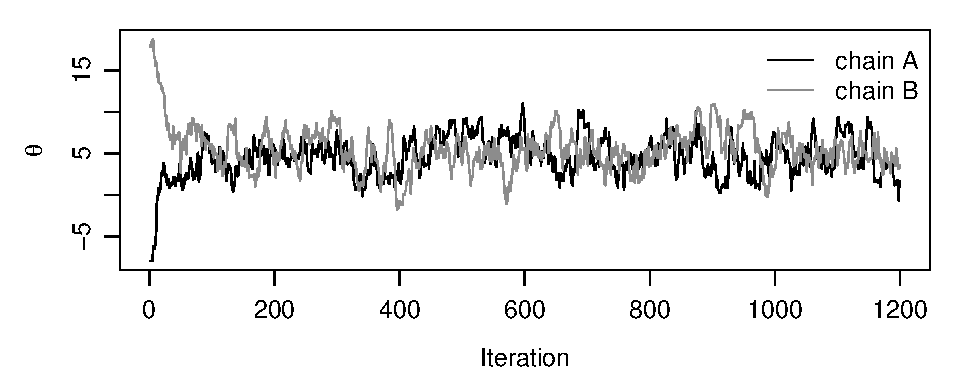
\includegraphics[width=0.7\linewidth]{r/out/q9_trace.pdf}
\end{center}
\R{d_q9.txt}

\begin{enumerate}
\item From the trace plot, how many initial iterations would you discard as burn-in? Explain in one or two sentences why burn-in is discarded.\mk{1}
\ans{1.5cm}
\item The Brooks--Gelman--Rubin statistic is $\hat R=B/W$, where $B$ is the standard deviation of the pooled draws from all chains and $W$ is the average of the within-chain standard deviations; the chains are judged converged if $\hat R<1.05$. Compute $\hat R$ for iterations 1--300 and for iterations 301--1200, and say what each tells you.\mk{2}
\ans{3cm}
\Needspace{8cm}
\item Use iterations 301--1200 of chain A ($n=900$ draws, sample standard deviation $s=2.29$) and the lag-1 autocorrelation in the output. Compute the effective sample size and the Monte Carlo standard error of the chain's sample mean. By what factor is the naive standard error $s/\sqrt n$ too small?\mk{2}
\ans{3cm}
\end{enumerate}

\clearpage
\section*{Additional working space}
\ans{20cm}
\end{document}
